 \documentclass{beamer}
\mode<presentation>
\usepackage{amsmath}
\usepackage{amssymb}
%\usepackage{advdate}
\usepackage{graphicx}
\usepackage{adjustbox}
\usepackage{subcaption}
\usepackage{enumitem}
\usepackage{multicol}
\usepackage{mathtools}
\usepackage{listings}
\usepackage{url}
\def\UrlBreaks{\do\/\do-}
\usetheme{Boadilla}
\usecolortheme{lily}
\let\vec\mathbf
\setbeamertemplate{footline}
{
  \leavevmode%
  \hbox{%
  \begin{beamercolorbox}[wd=\paperwidth,ht=2.25ex,dp=1ex,right]{author in head/foot}%
    \insertframenumber{} / \inserttotalframenumber\hspace*{2ex} 
  \end{beamercolorbox}}%
  \vskip0pt%
}
\setbeamertemplate{navigation symbols}{}

\providecommand{\nCr}[2]{\,^{#1}C_{#2}} % nCr
\providecommand{\nPr}[2]{\,^{#1}P_{#2}} % nPr
\providecommand{\mbf}{\mathbf}
\providecommand{\pr}[1]{\ensuremath{\Pr\left(#1\right)}}
\providecommand{\qfunc}[1]{\ensuremath{Q\left(#1\right)}}
\providecommand{\sbrak}[1]{\ensuremath{{}\left[#1\right]}}
\providecommand{\lsbrak}[1]{\ensuremath{{}\left[#1\right.}}
\providecommand{\rsbrak}[1]{\ensuremath{{}\left.#1\right]}}
\providecommand{\brak}[1]{\ensuremath{\left(#1\right)}}
\providecommand{\lbrak}[1]{\ensuremath{\left(#1\right.}}
\providecommand{\rbrak}[1]{\ensuremath{\left.#1\right)}}
\providecommand{\cbrak}[1]{\ensuremath{\left\{#1\right\}}}
\providecommand{\lcbrak}[1]{\ensuremath{\left\{#1\right.}}
\providecommand{\rcbrak}[1]{\ensuremath{\left.#1\right\}}}
\theoremstyle{remark}
\newtheorem{rem}{Remark}
\newcommand{\sgn}{\mathop{\mathrm{sgn}}}
\providecommand{\abs}[1]{\vert#1\vert}
\providecommand{\res}[1]{\Res\displaylimits_{#1}} 
\providecommand{\norm}[1]{\lVert#1\rVert}
\providecommand{\mtx}[1]{\mathbf{#1}}
\providecommand{\mean}[1]{E[ #1 ]}
\providecommand{\fourier}{\overset{\mathcal{F}}{ \rightleftharpoons}}
%\providecommand{\hilbert}{\overset{\mathcal{H}}{ \rightleftharpoons}}
\providecommand{\system}[1]{\overset{\mathcal{#1}}{ \longleftrightarrow}}
%\providecommand{\system}{\overset{\mathcal{H}}{ \longleftrightarrow}}
	%\newcommand{\solution}[2]{\vec{Solution:}{#1}}
%\newcommand{\solution}{\noindent \vec{Solution: }}
\providecommand{\dec}[2]{\ensuremath{\overset{#1}{\underset{#2}{\gtrless}}}}
\newcommand{\myvec}[1]{\ensuremath{\begin{pmatrix}#1\end{pmatrix}}}


\lstset{
%language=C,
frame=single, 
breaklines=true,
columns=fullflexible
}
\lstset{
  language=C,
  basicstyle=\ttfamily\footnotesize,
  keywordstyle=\color{blue}\bfseries,
  commentstyle=\color{gray}\itshape,
  stringstyle=\color{orange},
  numbers=left,
  numberstyle=\tiny\color{gray},
  breaklines=true,
  frame=single,
  showstringspaces=false,
  tabsize=4,
  captionpos=b
}
\numberwithin{equation}{section}
\lstset{
  language=Python,
  basicstyle=\ttfamily\small,
  keywordstyle=\color{blue},
  stringstyle=\color{orange},
  numbers=left,
  numberstyle=\tiny\color{gray},
  breaklines=true,
  showstringspaces=false
}

\title{Problem 12.113}
\author{Sujal Rajani}

\date{\today} 
\begin{document}

\begin{frame}
\titlepage
\end{frame}

\section{Question}
\begin{frame}{Question}
\textbf{Question }:
The area of the region bounded by the parabola \( y = x^2 + 1 \) and the straight line \( x + y = 3 \) is:
\\
\begin{enumerate}
    \item[\textbf{a)}] \( \frac{59}{6} \) 
    \\
    \item[\textbf{b)}] \( \frac{9}{2} \)
    \\
    \item[\textbf{c)}] \( \frac{10}{3} \)
    \\
    \item[\textbf{d)}] \( \frac{7}{6} \)
\end{enumerate}

\end{frame}
\begin{frame}{Solution}
\textbf{SOLUTION}
\textbf{Solution:}

\textbf{Step 1: Write equations in matrix (quadratic) form}
\begin{align*}
y &= x^2 + 1  \\
\text{In matrix form:} \quad \vec{x}^T 
\begin{pmatrix} 1 & 0 \\ 0 & 0 \end{pmatrix}
\vec{x} + 2
\begin{pmatrix} 0 \\ -\frac{1}{2} \end{pmatrix}^T
\vec{x} + 1 = 0
\end{align*}

     \end{frame}
     \begin{frame}{ Step-by-Step Calculation}    
\textbf{Step 2: Parametric representation of the line:} \\
\( x + y = 3 \implies y = 3 - x \) \\
Let the line in parametric vector form be:
\[
\vec{X} = \begin{pmatrix} 0 \\ 3 \end{pmatrix} + \lambda \begin{pmatrix} 1 \\ -1 \end{pmatrix}
\]

     \end{frame}
     \begin{frame}{ Step-by-Step Calculation}    

\textbf{Step 3: Substitute into the matrix equation and solve for \(\lambda\)}

Substitute \( x = \lambda,\, y = 3 - \lambda \) into the matrix equation.
\begin{align*}
\left(
\begin{pmatrix}
\lambda \\
3 - \lambda
\end{pmatrix}
\right)^T 
\begin{pmatrix}
1 & 0 \\
0 & 0
\end{pmatrix}
\begin{pmatrix}
\lambda \\
3 - \lambda
\end{pmatrix}
+ 2
\begin{pmatrix}
0 \\
-\frac{1}{2}
\end{pmatrix}^T 
\begin{pmatrix}
\lambda \\
3 - \lambda
\end{pmatrix}
+ 1 = 0
\end{align*}
\end{frame}
\begin{frame}{Frame Title}
    Calculate each component:
\begin{align*}
& \begin{pmatrix}
\lambda \\
3 - \lambda
\end{pmatrix}^T 
\begin{pmatrix}
1 & 0 \\
0 & 0
\end{pmatrix}
\begin{pmatrix}
\lambda \\
3 - \lambda
\end{pmatrix}
= \lambda^2 \\
& 2\begin{pmatrix}
0 \\
-\frac{1}{2}
\end{pmatrix}^T 
\begin{pmatrix}
\lambda \\
3 - \lambda
\end{pmatrix}
= 2 \cdot \left(0 \cdot \lambda + \left(-\frac{1}{2}\right) (3 - \lambda) \right)
= - (3 - \lambda) = -3 + \lambda
\end{align*}
So, the equation becomes:
\[
\lambda^2 - 3 + \lambda + 1 = 0 
\implies \lambda^2 + \lambda - 2 = 0
\]
Solving this quadratic equation:
\[
(\lambda + 2)(\lambda - 1) = 0 \implies \lambda = -2,\, 1
\]
So, the intersection points are:
\[
\vec{X} = \myvec{-2\\ 5} , \vec{X} = \myvec{1\\2}
\]


\end{frame}

     
     \begin{frame}{ Step-by-Step Calculation}    
\textbf{Step 4: Area Calculation}

The area between the curves can be written as:
\[
A = \int_{-2}^{1} \left[ (3-x) - (x^2 + 1) \right] \, dx = \int_{-2}^{1} (2 - x - x^2)\, dx
\]

Integrate:
\begin{align*}
A &= \int_{-2}^{1} (2 - x - x^2)\,dx \\
&= \left[ 2x - \frac{1}{2}x^2 - \frac{1}{3}x^3 \right]_{-2}^{1}\\
&= \left(2(1) - \frac{1}{2}(1)^2 - \frac{1}{3}(1)^3\right) - \left(2(-2) - \frac{1}{2}(-2)^2 - \frac{1}{3}(-2)^3\right) \\
&= (2 - 0.5 - 0.333) - (-4 - 2 + 2.666) \\
&= 1.167 - (-3.334) \\
&= 4.5 = \frac{9}{2}
\end{align*}
 \end{frame}

    \begin{frame}[fragile]
    \begin{figure}[H]
    \centering
    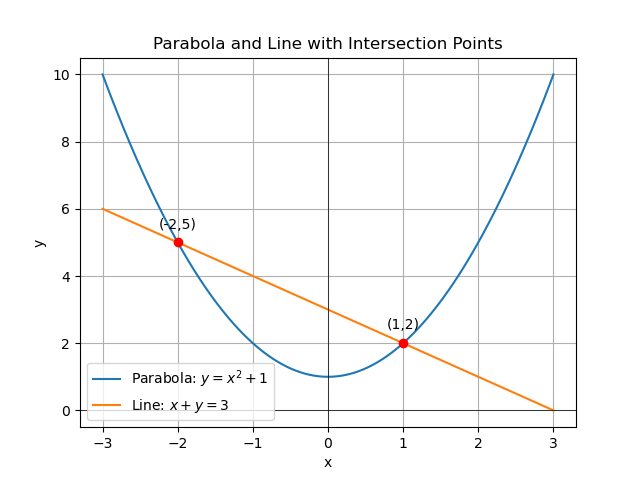
\includegraphics[width = 0.6\columnwidth]{../figs/img.png}
    \caption*{}
    \label{figs}
\end{figure}
\end{frame}

\end{document}